    \documentclass[a4paper]{article}
\usepackage{blindtext}
\usepackage[T1]{fontenc}
\usepackage{lmodern}
\usepackage[utf8]{inputenc}
\usepackage[unicode]{hyperref}
\usepackage{amsfonts}
\usepackage{amsmath}
\usepackage{graphicx}
\usepackage{outlines}
\usepackage{pdfpages}
\usepackage{geometry}
\usepackage{svg}
\usepackage{mathtools}
\usepackage{enumitem}
\usepackage{amsthm}
\usepackage{titlesec}
\usepackage{float}
\usepackage{enumitem}
\usepackage{array}
\usepackage{color, colortbl}
\usepackage{graphicx}
\usepackage{subcaption}
\usepackage{mwe}
\usepackage[ruled,vlined]{algorithm2e}
\usepackage{biblatex}
\addbibresource{p.bib}


\newcommand*{\naturalNumbers}{\mathbb{N}}%

\title{Hate speech classification}
\author{Paweł Flis, Karol Krupa, Rafał Chabasiński}
\date{April 2022}

\begin{document}
\maketitle

\section{Introduction}
Social media platforms such as Facebook, Twitter, Instagram and YouTube are experiencing a continuous growth in number of users. In recent years, partially due to COVID-19 pandemic even older generations turned to those platforms as a way to experience wider range of human interactions. Along with all the advantages social media brings, there are number of hazards related to harmful actions of some of its users encouraged by their perceived anonymity.
\par
Especially recently hate speech has been under the scope of investigation to make the internet a safe and welcoming space for everyone. This topic garnered scientific attention due to the potential of applying machine learning for hate speech recognition, which would in turn help counteract cyberbullying. Although the very idea of using automatic censors is highly questionable their counselling can be of invaluable aid. In this case the hate speech detector accuracy is of the essence as too rigorous model could severely affect freedom of expression while high-tolerance one would maintain unsafe environments.
\section{Literature analysis}
Number of Natural Language Processing in conjunction with Deep Learning solutions have been proposed during the years, however majority of these solutions requires great amount of labelled data, which has to be manually labeled by a human, which eventually which limits the cognitive capabilities of the model. It is also really hard to identify semantic nuances which often decide on the overall sentiment. There also have been attempts to tackle the problem using statistical models such as n-grams, SVM or Linear Regression.
\par
Bidirectional Encoder Representations from Transformers model has shown a great prowess in various NLP tasks, in many cases outperforming its predecessors.
Mozafari et al.~\cite{paper} proposed a semi-supervised solution based on pre-trained BERT model with broad contextual knowledge and using transfer learning to fine tune a model on labelled samples from target domain of hate speech. 
\par
This approach considers two variants of BERT networks. $BERT_{base}$ having 12 layers and 110 million parameters and $BERT_{large}$ hacing double the layers and triple the parameters. The output is a sentence representation in a 768-dimensional vector, which is an input to domain specific classifier.
\par
In paper number of fine-tuning approaches are presented:
\begin{enumerate}
    \item \textbf{BERT based fine-tuning} \\
    $BERT_{base}$ model with one fully connected layer at the top and softmax activation function with no hidden layers.
    \item \textbf{Insert nonlinear layers} \\
    $BERT_{base}$ model with multilayer perceptron with two hidden layers at the top level.
    \item \textbf{Insert Bi-LSTM layer} \\
    $BERT_{base}$ model with Bi-LSTM recurrent neural network and one fully connected layer on the output.
    \item \textbf{Insert CNN layer} \\
    Output of each transformer from $BERT_{base}$ is concatenated to produce a matrix that is an input to CNN, later max pooling is performed and output is deduced using one fully connected layer once agian.
\end{enumerate}
\par
The authors performed data pre-processing to make the text input data more suitable for BERT model - emoticons were changed into <tags>, multiple word hashtags were separated and everything has been turned into lowercase. It is important to notice, that by doing that some relevant information may be lost, however we trust that it is a calculated decision and it is of benefit to used BERT model.
\par
Version with CNN layer proved to perform the best across all metrics (Precision, Recalll, F1-score). It outperformed other solutions designed for the very same datasets used in  ~\cite{ref1}~\cite{ref2}~\cite{ref3}. It is worth noting that BERT with nonlinear layers performed surprisingly poorly(much worse than with no hidded layers) on dataset with samples labelled as Hate[1430] Offensive[19190] Neither[4163] so dataset heavily biased towards 'just' offensive content.

\newpage
\section{Exploratory data analysis}
\subsection{Data examples}
\begin{itemize}
    \item non-harmful
        \begin{itemize}
            \item anonymizedaccount anonymizedaccount Zaległości były, ale ważne czy były wezwania do zapłaty z których się klub nie wywiązał.
            \item anonymizedaccount Tym w sejmie też? Banda hipokrytów i złodziei.
        \end{itemize}
    \item cyberbullying
        \begin{itemize}
            \item anonymizedaccount anonymizedaccount Czas pokaże kto jest kim, mącicielu, szkodniku, haha do gazu haha
            \item anonymizedaccount anonymizedaccount anonymizedaccount Pis mial być inny, jesteś idiotą
        \end{itemize}
    \item hate-speech
        \begin{itemize}
            \item RT anonymizedaccount anonymizedaccount Pasujecie do siebie antypolskie kanalie.
            \item anonymizedaccount Pierwszy priorytet zadowolić Jarkacza, drugi priorytet ssać kasę wszystkimi otworami,  mają rozdwojenie jaźni
        \end{itemize}
\end{itemize}

We can see that subjects are anonymized and are easily recognizable, which will be helpful for our algorithms.

\newpage
\subsection{Label data split}
\begin{figure}[h]
\centering
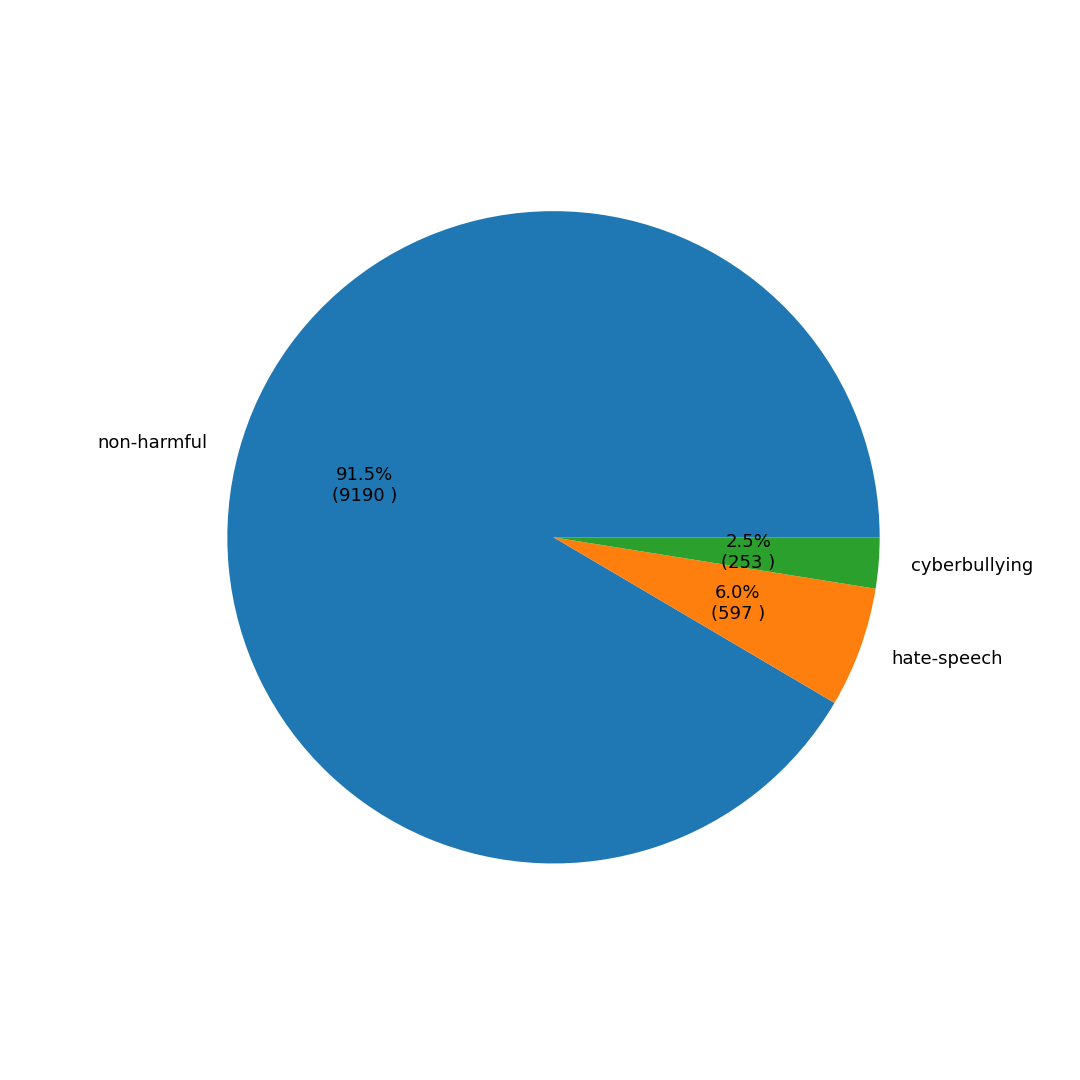
\includegraphics[width=\textwidth]{plots/tags_pie_plot.png}
\caption{Labels distribution}
\end{figure}

\newpage
\subsection{Data attributes}
\begin{figure}[H]
\centering
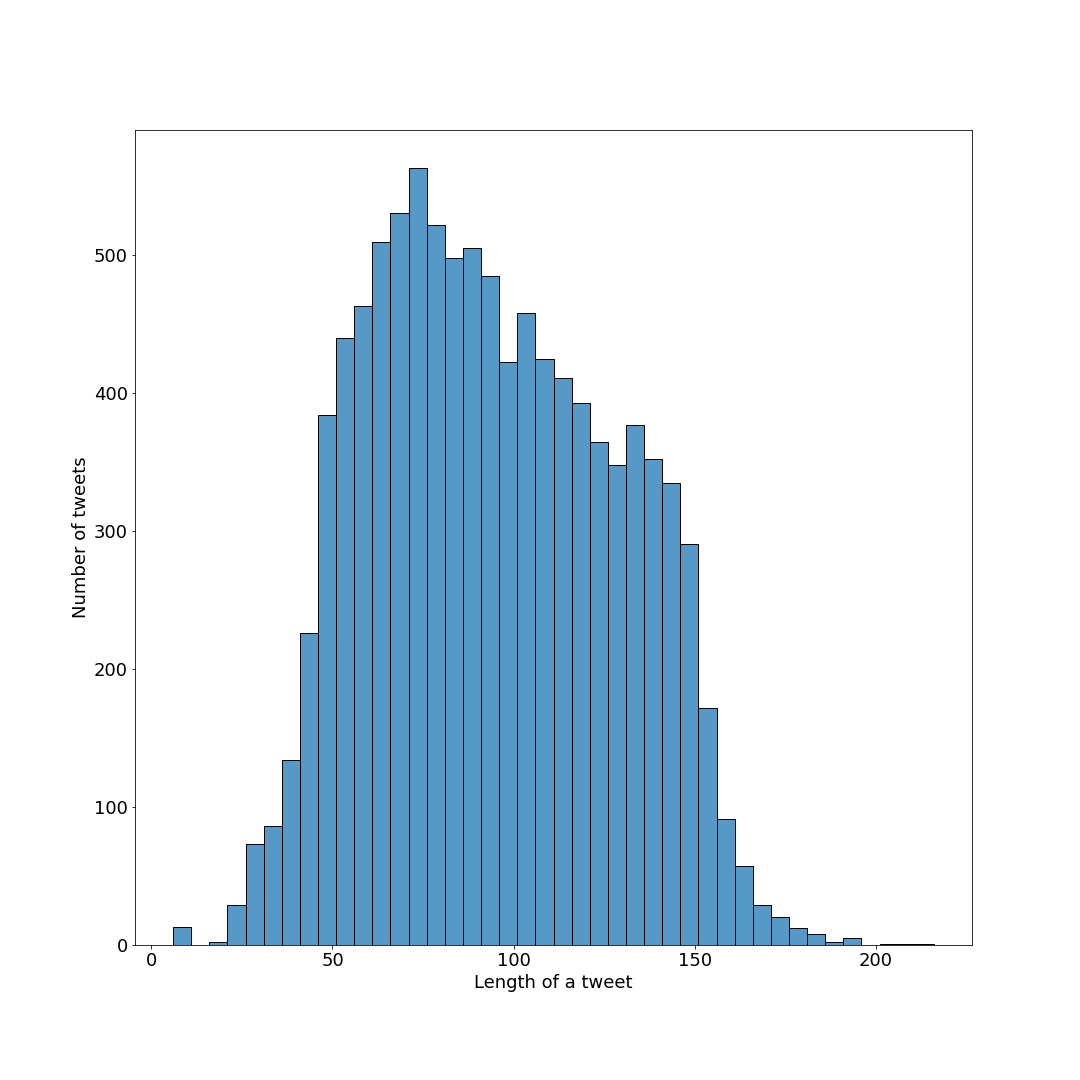
\includegraphics[width=\textwidth]{plots/tweet_lengths_plot.png}
\caption{Tweets lengths}
\end{figure}

\begin{figure}[H]
\centering
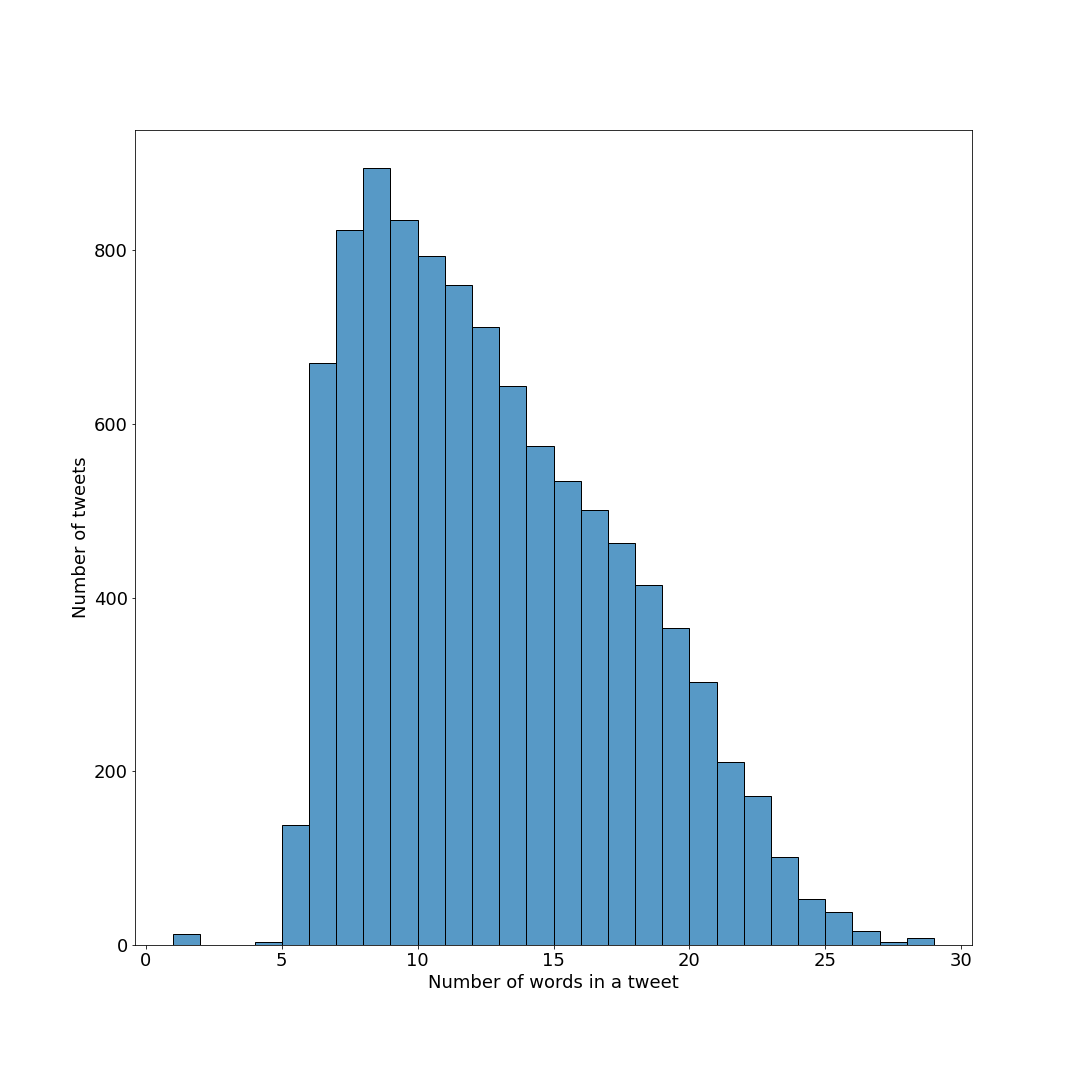
\includegraphics[width=\textwidth]{plots/tweet_word_counts_plot.png}
\caption{Tweets word counts}
\end{figure}

\begin{figure}[H]
\centering
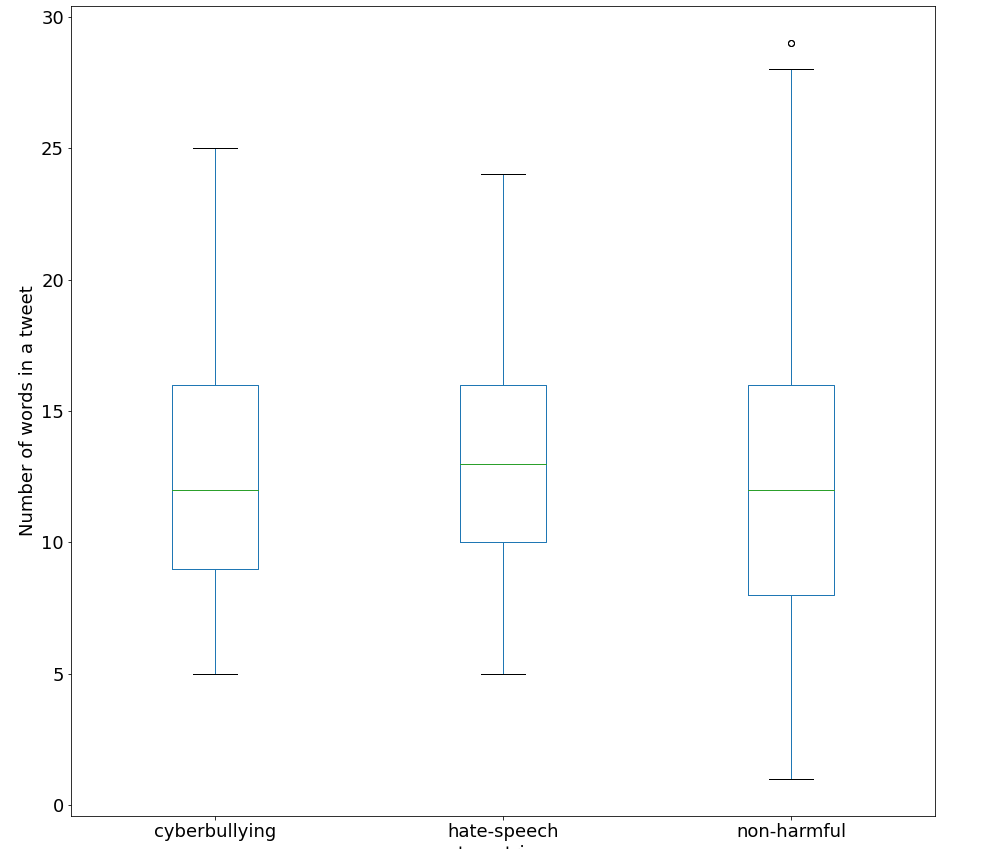
\includegraphics[width=\textwidth]{plots/tweet_word_counts_box_plot.png}
\caption{Tweets word counts box plot for different labels}
\end{figure}

\newpage
\section{Solution concept}

Preparing our solution to the problem is to prepare a program that, given an expression written by a human, returns a result of 1 if the statement is hate-filled and 0 otherwise. 

In order to perform this task as well as possible, we need to:
\begin{enumerate}
    \item Properly transfer expressions and sentences into a form understandable by a computer - that is, vectorize them using an appropriate tokenizer. 
    \item Model the language and its internal dependencies using certain language models.
    \item Train the language models for our task, which is hate speech recognition.
\end{enumerate}

The first two steps can be solved by choosing a pretrained model. A collection of such models is available at this link \href{https://klejbenchmark.com/leaderboard/}{KLEJ-Benchmark}.
The first two steps are strongly related, since the trained model has been trained for selected embeddings and is unlikely to work for others.

An example model from the list above is HerBERT \cite{mroczkowski-etal-2021-herbert} and XLM-RoBERTa \cite{dadas2020pretraining}. Both score very high on the CBD task \cite{ptaszynski2019results}, which is the task we solve. For this reason, we decided to select pre-trained models and then retrain them for our purposes.
In addition, for the second model, the authors provided scripts that give the ability to train the model to a specific KLEJ-benchmark problem, including the CBD problem. The scripts are available here: \href{https://github.com/sdadas/polish-roberta}{scripts}.

The computations will be done with google cloud graphics cards, on the google collab site. Verification will be done using Precision, Recalll, F1-score metrics.

\printbibliography

\end{document}
 